% !TEX program = pdflatex
\documentclass[twocolumn,reprint,aps,prd,floatfix,amsmath,amssymb]{revtex4-2}

\usepackage{amsmath,amssymb}
\usepackage{booktabs}
\usepackage{graphicx}
\usepackage{xcolor}
\usepackage{tikz}
\usetikzlibrary{arrows.meta,bending}
\graphicspath{{../figures/quovar/}}

\begin{document}

\title{Quovar: History-Shaped Quantum Walk Steps with Adaptive Register Grids}

\author{Amelia Fargason}
\email{afargason3@gatech.edu}
\affiliation{School of Physics, Georgia Institute of Technology, Atlanta, Georgia 30332, USA}
\affiliation{School of Mathematics, Georgia Institute of Technology, Atlanta, Georgia 30332, USA}

\author{Rasmit Devkota}
\email{rdevkota3@gatech.edu}
\affiliation{School of Physics, Georgia Institute of Technology, Atlanta, Georgia 30332, USA}
\affiliation{School of Mathematics, Georgia Institute of Technology, Atlanta, Georgia 30332, USA}

\date{\today}

\begin{abstract}
We study a coherent circuit that generates random-walk steps with covariance proportional to the covariance of a finite history. The circuit builds each step from signed differences between pairs of history states, so it does not first calculate and store a covariance matrix. We combine this construction with an adaptive register grid (AMR), which uses measurements from one circuit run to choose a local grid for the next run. In a two-dimensional test with three history states, finite-grid QCLT steps have a median relative covariance error of 8.77\%, compared with 3.97\% when the grid is selected by AMR. Across seven synthetic step geometries, AMR improves five cases that are poorly resolved by a fixed local grid and is less accurate in two cases that the fixed grid already resolves. The eight-bit coherent example uses 33 logical qubits, including preparation of its known-mode history. These results characterize history-shaped quantum steps and the effect of grid resolution on their covariance.
\end{abstract}
\maketitle

\section{Introduction}

Markov chain Monte Carlo (MCMC) methods generate a sequence of states to explore a probability distribution. In Bayesian inference, that distribution is often a posterior. At each step, the method proposes a new state and uses an acceptance rule to decide whether the chain moves there. The proposal's scale and orientation affect how quickly the chain explores the target, especially when different directions have different characteristic widths.

BayesWave motivates part of this work. It reconstructs gravitational-wave bursts and instrumental glitches with a variable number of Morlet--Gabor wavelets and reversible-jump MCMC \cite{cornish2015bayeswave,becsy2017parameter}. A sine-Gaussian wavelet has five intrinsic parameters, but the full BayesWave model is not a fixed five-dimensional problem: the number of wavelets can change, and the signal and detector models add further structure. Here we use small synthetic walks to study history-shaped proposals and finite register grids.

This paper focuses on two components. The first is a coherent QCLT circuit that generates a step with covariance proportional to the covariance of stored history. The second is an adaptive mesh refinement (AMR) rule that chooses the center, orientation, and spacing of a fixed-width register grid from earlier circuit samples. We measure how closely these steps reproduce their intended covariance, compare them with covariance readout methods, and examine when AMR improves on a fixed local grid.

Adaptive proposals have a long history in classical MCMC. Adaptive Metropolis uses the covariance of past states to set proposal shape \cite{haario2001adaptive}, and differential-evolution MCMC uses differences between stored states \cite{terbraak2008demcz}. Adaptive tempered reversible-jump methods also combine proposal adaptation with changing model dimension \cite{tian2024adaptive}. Quantum-walk formulations of Metropolis--Hastings address a larger algorithmic problem than step generation alone \cite{lemieux2020efficient}. The circuit studied here generates a history-shaped proposal step; the numerical experiments below evaluate that component.

\section{History-conditioned QCLT step}

Let $h_1,\ldots,h_K\in\mathbb{R}^d$ be $K$ stored positions, with mean $\bar h$ and unbiased sample covariance
\begin{equation}
  S_h=\frac{1}{K-1}\sum_{a=1}^{K}(h_a-\bar h)(h_a-\bar h)^{\mathsf T}.
\end{equation}
The pair-difference identity
\begin{equation}
  \sum_{a<b}(h_a-h_b)(h_a-h_b)^{\mathsf T}=K(K-1)S_h
\end{equation}
provides a direct way to generate a step with this covariance. For independent signs $r_{ab}\in\{-1,+1\}$, define
\begin{equation}
  \Delta=\gamma\sum_{a<b}r_{ab}(h_a-h_b),\qquad
  \gamma=\sqrt{\frac{2.38^2/d}{K(K-1)}}.
\end{equation}
Conditioned on the history, $\mathbb{E}[\Delta]=0$ and
\begin{equation}
  \operatorname{Cov}(\Delta\mid h_1,\ldots,h_K)=\frac{2.38^2}{d}S_h.
\end{equation}
The equality describes the second moment. With finitely many history pairs and sign bits, the step distribution is discrete and need not be Gaussian. The same distribution can also be sampled classically by drawing the pair signs.

We study two circuit settings. In the known-mode walk, preparation signs encode the history states coherently, and the step uses those same signs. This construction applies to the specified walk with known initial position and displacement modes. In the compiled circuit, history values are supplied as classical gate constants; the output step is coherent, while the history is classical.

For the two-dimensional example, $K=3$ and each coordinate has an eight-bit position register. The known-mode circuit uses 33 logical qubits: 16 position qubits, 6 history-preparation sign qubits, 6 pair-selection and pair-sign qubits, 4 isotropic-step qubits, and 1 parity qubit. A full-strength compiled step with classical history uses 21 qubits, and a lazy compiled step uses 24. The additional qubits in the 33-qubit circuit prepare the known-mode history coherently.

\begin{figure*}[!t]
\centering
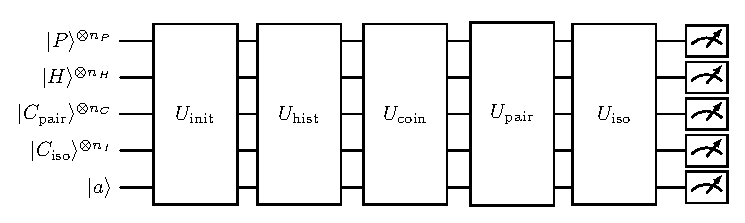
\includegraphics[width=0.90\textwidth]{qclt_amr_circuit.pdf}
\caption{Coherent known-mode QCLT step circuit for the two-dimensional example. The five registers hold position, history-preparation signs, pair-step choices, isotropic-step choices, and a parity ancilla. Each register contains the indicated number of qubits for the $K=3$, eight-bit example.}
\label{fig:qclt-circuit}
\end{figure*}

\section{Adaptive register grid}

Each coordinate is represented by a fixed number of register bits. A grid spanning a wide range has coarse spacing; a grid covering a smaller region represents local steps more finely. AMR uses samples from one circuit execution to estimate a window center and principal axes, then selects the grid spacing for a later execution. The samples are measured between circuit runs, and the next run is compiled for the updated grid.

\begin{figure*}[!t]
\centering
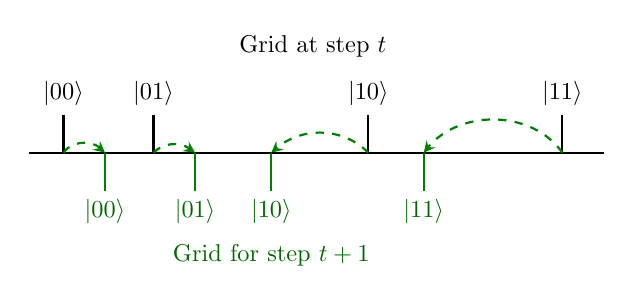
\begin{tikzpicture}[>=stealth,scale=0.88, every node/.style={transform shape}]
  \draw[thick] (-0.5,0) -- (7.8,0);
  \foreach \x/\lab in {0/00,1.3/01,4.4/10,7.2/11} {
    \draw[thick] (\x,0) -- (\x,0.55);
    \node[above] at (\x,0.55) {$|\lab\rangle$};
  }
  \foreach \x/\lab in {0.6/00,1.9/01,3.0/10,5.2/11} {
    \draw[thick,green!50!black] (\x,0) -- (\x,-0.55);
    \node[below,text=green!40!black] at (\x,-0.55) {$|\lab\rangle$};
  }
  \draw[->,dashed,thick,green!50!black] (0,0) to[bend left=55] (0.6,0);
  \draw[->,dashed,thick,green!50!black] (1.3,0) to[bend left=45] (1.9,0);
  \draw[->,dashed,thick,green!50!black] (4.4,0) to[bend right=45] (3.0,0);
  \draw[->,dashed,thick,green!50!black] (7.2,0) to[bend right=55] (5.2,0);
  \node[above] at (3.6,1.25) {Grid at step $t$};
  \node[below,text=green!40!black] at (3.0,-1.2) {Grid for step $t+1$};
\end{tikzpicture}
\caption{AMR changes the center and spacing of the coordinate grid between circuit executions. The same register labels therefore represent different physical values on successive runs.}
\label{fig:amr-grid}
\end{figure*}

We use $\kappa$ for the window width in units of recent standard deviations. The refinement rule must balance resolution against coverage: a narrow window gives finer local spacing but can exclude relevant parts of the target, while a wide window covers more of the target at lower resolution. The AMR comparisons below use a sample-based window and check whether all history states and possible pair steps remain inside it.

\section{Results}

\subsection{QCLT steps and covariance readout}

The covariance experiment enumerates 64 branches of a two-dimensional walk with three preparatory steps along known modes. Direct QCLT steps have a median relative covariance error of 8.77\% across branches, with a 10th--90th percentile range of 6.66--9.17\%. This error comes from representing the step on a finite grid. At 384 measurement shots, pairwise moments give 11.76\% median error and SWAP overlap gives 9.29\%. The SWAP estimate is already close to direct QCLT at this measurement budget. Readout methods estimate covariance entries, then require a separate step-preparation circuit.

\begin{figure*}[!t]
\centering
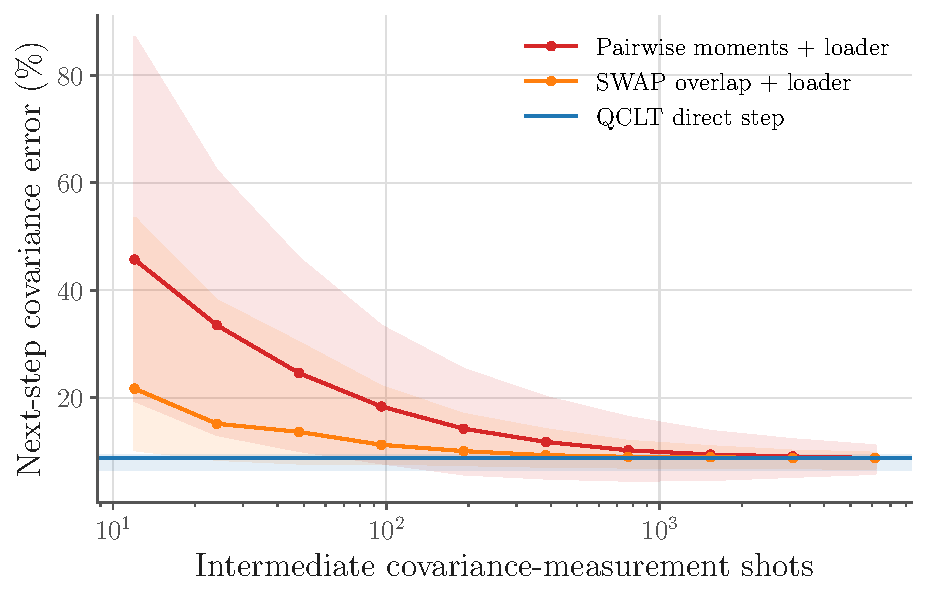
\includegraphics[width=0.86\textwidth]{qclt_step_generation.pdf}
\caption{Relative covariance error of direct QCLT steps and measurement-based covariance pipelines versus measurement budget. The QCLT error is due to finite-grid representation; readout methods include finite-shot error.}
\label{fig:step-generation}
\end{figure*}

Table~\ref{tab:covariance-method-errors} gives the full comparison and the error distributions for each method. The classical AM and DE-MCz reference receives exact history covariance, so its error is zero by construction.

\begin{table*}[!t]
\centering
\small
\caption{Relative next-step covariance error for all methods in the comparison. $N$ is the number of branch, window, or measurement-repetition error samples, as appropriate. Readout methods use 384 total shots or queries and assume an ideal step loader.}
\label{tab:covariance-method-errors}
\input{figures/covariance_method_errors.tex}
\end{table*}

\subsection{When AMR improves covariance representation}

We test seven two-dimensional step geometries: tilted, axis-aligned, anti-tilted, isotropic, broader, grid-aligned, and isotropic-exact. On the first five, the eight-bit AMR grid improves covariance error over the informed local grid. AMR median errors range from 2.61\% to 5.50\% across those cases. On the two cases already well represented by the local grid, AMR is less accurate: the local-grid errors are 0.114\% and 0.083\%, compared with 4.88\% and 5.12\% for AMR. Thus, AMR helps when the fixed grid poorly resolves the step geometry, while a well-chosen fixed grid can be more accurate when it already matches the target.

\begin{figure*}[!t]
\centering
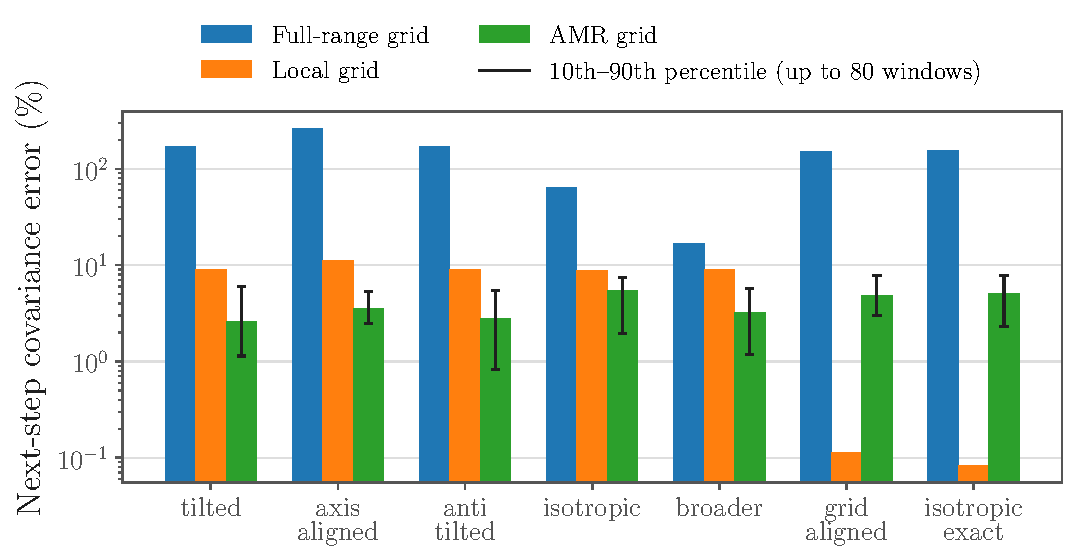
\includegraphics[width=0.92\textwidth]{qclt_amr_covariance_error.pdf}
\caption{Relative next-step covariance error for full-range, informed local, and AMR grids across seven geometries. AMR intervals span the 10th--90th percentiles of safe sample-selected windows.}
\label{fig:amr-error}
\end{figure*}

The AMR window is estimated from 8 to 1,000 samples. For each sample count and geometry, we test 80 independently selected subsets from a 20,000-sample pool. With 1,000 samples, AMR improves on the local grid in 99--100\% of trials for the five under-resolved cases. It does not improve the two cases that the local grid already resolves accurately.

\begin{figure*}[!t]
\centering
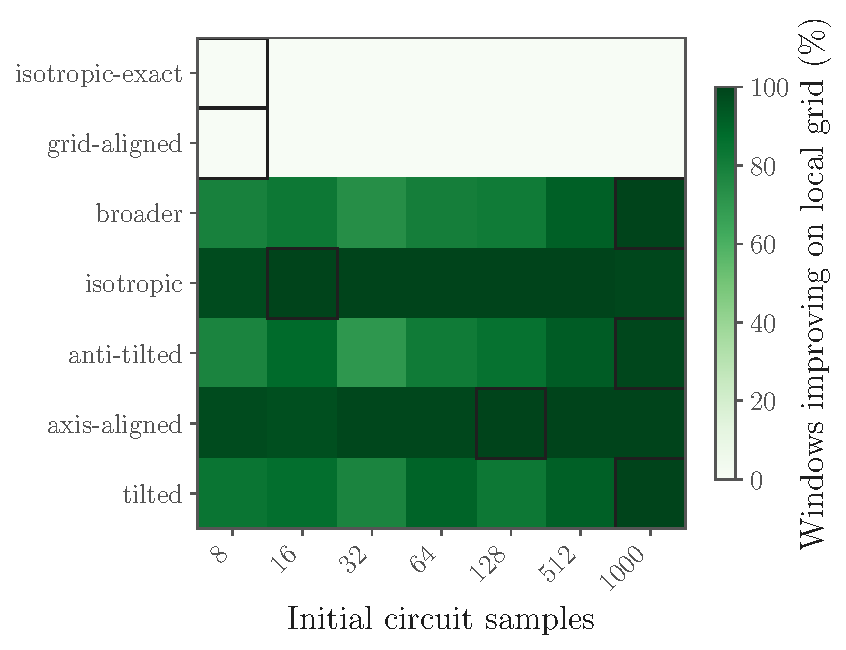
\includegraphics[width=0.72\textwidth]{qclt_amr_pilot_success.pdf}
\caption{Fraction of sample-selected AMR windows with lower covariance error than the informed local grid, by geometry and number of initial circuit samples.}
\label{fig:amr-sample-count}
\end{figure*}

The tilted test has the same covariance eigenvalues as its axis-aligned counterpart but different principal directions. The comparison below shows why a grid aligned with the covariance can help represent a correlated step using a limited number of bits.

\begin{figure*}[!t]
\centering
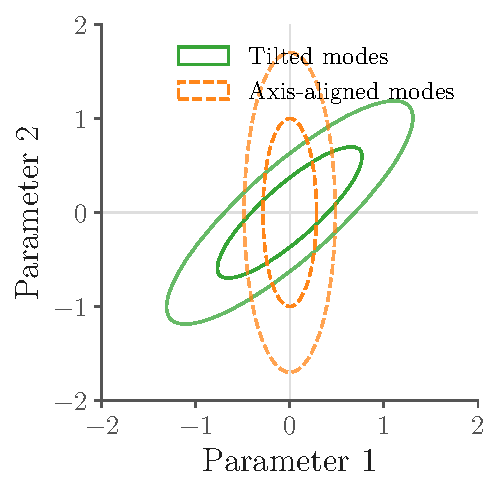
\includegraphics[width=0.48\textwidth]{qclt_amr_tilted_geometry.pdf}
\caption{Tilted and axis-aligned covariance contours with identical eigenvalues. The tilted principal directions are not aligned with the coordinate axes.}
\label{fig:tilted-geometry}
\end{figure*}

\subsection{AMR refinement choices}

We also vary the interval between grid updates, the edge-occupancy threshold that triggers widening, the maximum width change, and the fraction of the recent mean shift used to move the window. These tests use six random seeds on a narrow target and a two-mode target. For the two-mode case, median occupancy of the higher-probability peak decreases from 0.945 when the grid is updated every 200 steps to 0.919 when it is updated every 1,600 steps. The edge threshold has little effect over the tested range, and the narrow-target error does not have a stable optimum across six seeds. The best settings therefore depend on the target and should be reported with the problem and sample budget.

\begin{figure*}[!t]
\centering
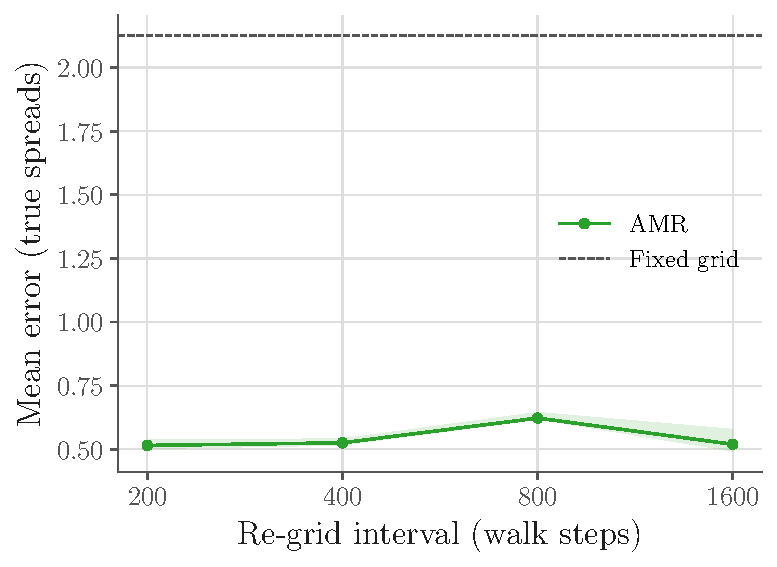
\includegraphics[width=0.72\textwidth]{amr_regrid_interval_narrow.pdf}
\caption{Narrow-target error versus the number of walk steps between AMR grid updates. Shading shows the interquartile range across six seeds.}
\label{fig:regrid-narrow}
\end{figure*}

\begin{figure*}[!t]
\centering
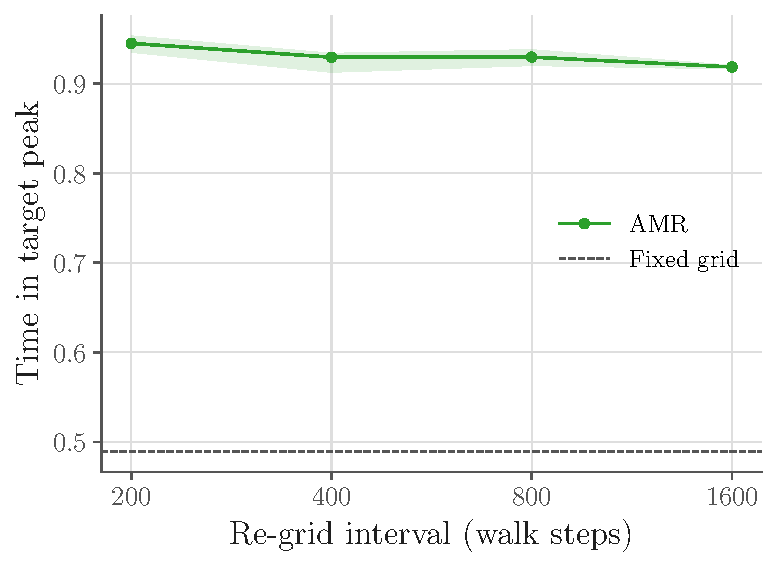
\includegraphics[width=0.72\textwidth]{amr_regrid_interval_decoy.pdf}
\caption{Higher-probability peak occupancy versus the number of walk steps between AMR grid updates for the two-mode target.}
\label{fig:regrid-two-mode}
\end{figure*}

\begin{figure*}[!t]
\centering
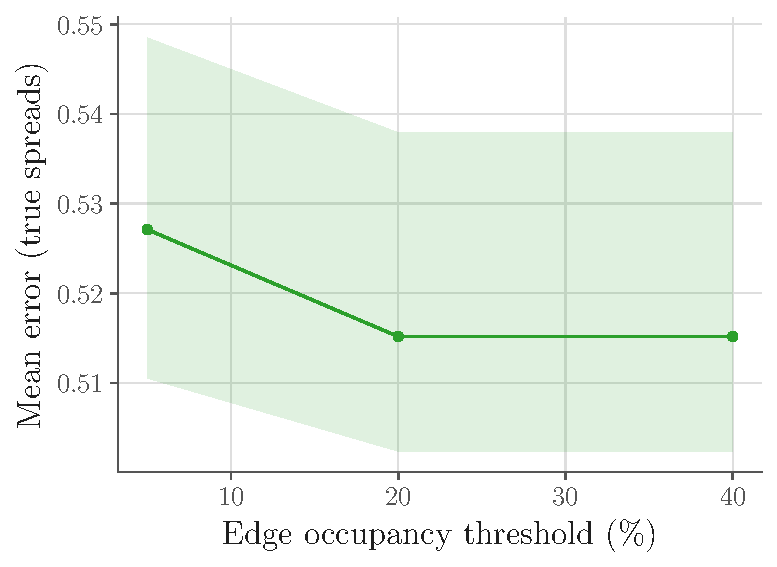
\includegraphics[width=0.72\textwidth]{amr_edge_threshold_narrow.pdf}
\caption{Narrow-target error versus the edge-occupancy threshold used to trigger window widening.}
\label{fig:edge-narrow}
\end{figure*}

\begin{figure*}[!t]
\centering
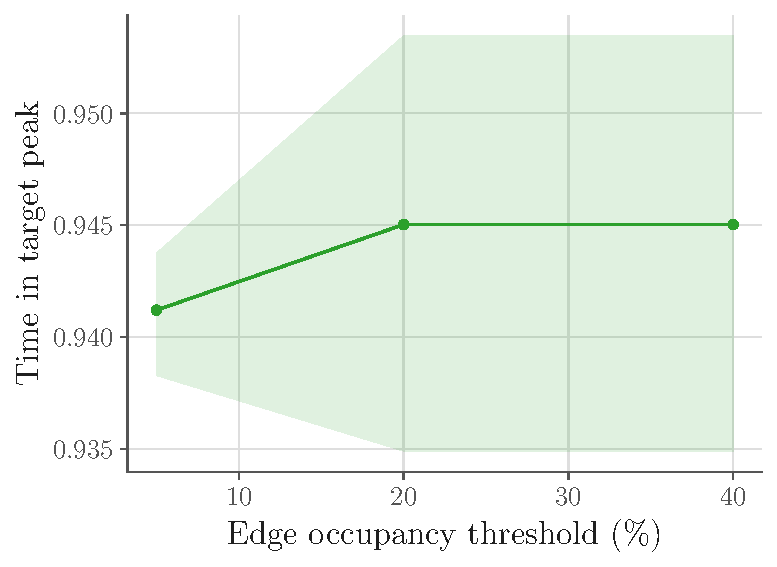
\includegraphics[width=0.72\textwidth]{amr_edge_threshold_decoy.pdf}
\caption{Higher-probability peak occupancy versus the edge-occupancy threshold for the two-mode target.}
\label{fig:edge-two-mode}
\end{figure*}

\begin{figure*}[!t]
\centering
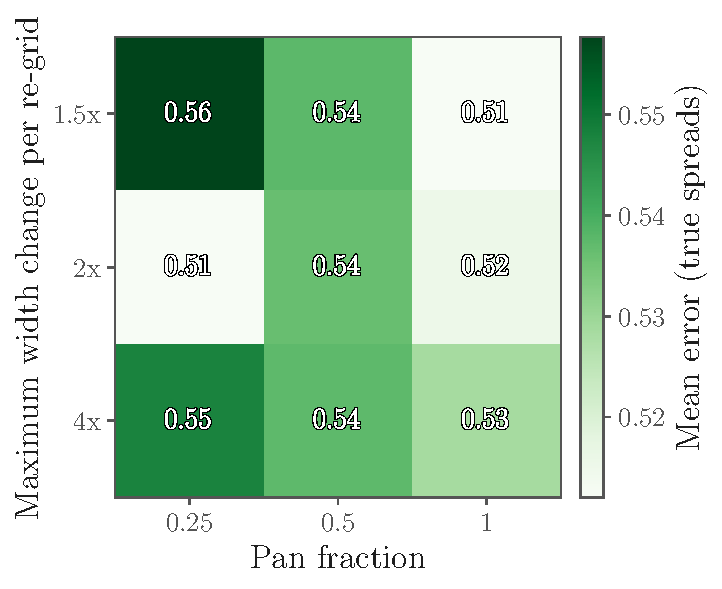
\includegraphics[width=0.72\textwidth]{amr_zoom_pan_narrow.pdf}
\caption{Narrow-target error as the maximum window-width change and fraction of recent mean shift are varied.}
\label{fig:zoom-pan-narrow}
\end{figure*}

\begin{figure*}[!t]
\centering
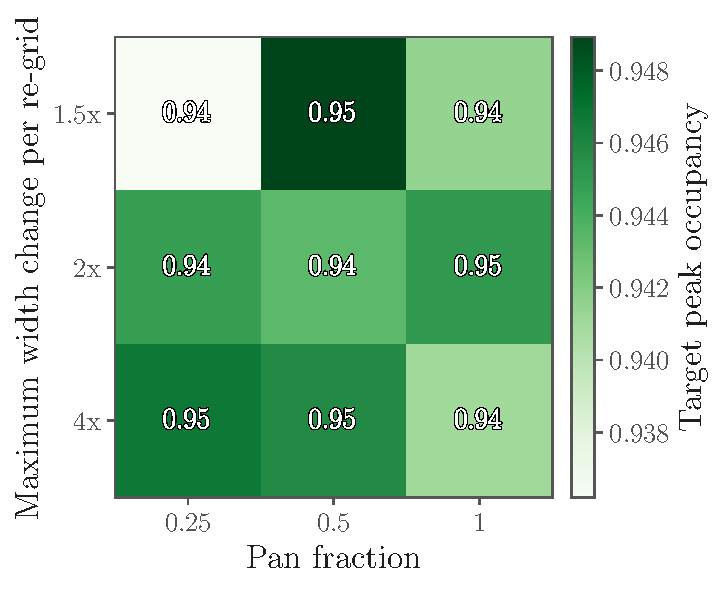
\includegraphics[width=0.72\textwidth]{amr_zoom_pan_decoy.pdf}
\caption{Higher-probability peak occupancy as the maximum window-width change and fraction of recent mean shift are varied for the two-mode target.}
\label{fig:zoom-pan-two-mode}
\end{figure*}

\section{Discussion}

The QCLT construction generates a step with a conditional covariance set by history pair differences. Its finite register introduces a measurable covariance error, and the step distribution remains discrete. AMR can reduce that error when a fixed grid is poorly matched to the step geometry by centering and orienting the available grid around sampled history. The same adaptation can add error when an informed fixed grid already represents the target well.

The reported qubit counts cover proposal generation for the examples studied here. Connecting the step circuit to a complete sampler, including its target evaluation and acceptance rule, is the next resource-cost question.

\section{Conclusion}

We evaluated a coherent history-covariance step and a sample-updated register grid on small synthetic walks. Pairwise history differences give the desired conditional covariance without explicitly constructing its matrix. AMR improves finite-grid covariance accuracy on several under-resolved geometries, and the tests also show cases where a fixed informed grid is better. The next step is to connect these proposal circuits to a complete sampler and test the resulting method on more realistic targets.

\bibliographystyle{apsrev4-2}
\bibliography{references}

\end{document}
